\documentclass[../main.tex]{subfiles}

\graphicspath{{\subfix{../images/}}}



\begin{document}



\clearpage
\thispagestyle{empty}
\vspace*{7cm}
\section{LAB 05 - May 19th}
\vspace*{1.5cm}


The following section and subsections are representative of a possible solution for the laboratory given for this course on May 19th 2026.
The version you find below might differ from what was submitted and it might differ from what is now being asked. 


\vspace*{1cm}
\subsection{Introduction}

In this laboratory, we will use a MCU by interacting with sensors and external peripherals, the microcontroller enables the acquisition, processing, and management of data from the surrounding environment. 
During the experimental activity, the main functions of the MCU will be explored, putting into practice programming and data acquisition concepts, such as monitoring physical parameters like ambient temperature.

\subsubsection*{Objective}

This laboratory has the goal of measuring the ambient temperature using an NTC thermistor, and to display the result on the builtin LCD screen of the VirtLAB board.

The laboratory report describes the structure and implementation of the firmware developed for the previous laboratory and it is structured around three concurrent tasks that comunicate using message queues.


\subsubsection*{Instruments} 

For the accomplishment of this task the following instruments and hardware components where used:

\begin{enumerate}[label=\textbf{-}]
	\item NTC Resistor - 10 k$\Omega$ at 25$^\circ$C, decreasing by 4\% per $^\circ$C rise.
	\item 3 x 10 k$\Omega$ resistors
	\item Agilent 34410A 6 1/2 digit multimeter.
	\item VirtLAB Board
	\item Mounting equipment (i.e. breadboard, jumper cables, ect.)
\end{enumerate}


\subsubsection*{Observations}

During the laboratory we first developed a firmware that implemented inside the \texttt{acquisition.c} the full acquisition and computation of the temperature value. Since we decided that using that much resources to compute each time (logarithmic function) we implemented a simple LUT and relative functions that returns a temperature value. The LUT was generated outside the MCU and is just stored in \texttt{.roadata} which is stored in flash memory and not loaded into RAM.\\

Inside the submitted project the old implementation is still visible but commented out.

\subsubsection*{Problems}


During this laboratory no serious problems or error were encountered.
Also in the laboratory papers states to measure the voltage supply to fix any possible reading; this operation is no longer necessary as it is the same voltage source for both voltage dividers, this il clearly visible in the equations inside the laboratory papers.











\subsection{Hardware}

We begin no describing the hardware configuration of the different devices used for the temperature measurement.\\

\subsubsection*{NTC Resistor and Voltage Divider}

Temperature is calculated using the resistance of an NTC thermistor, whose resistance changes with temperature. The component has a nominal resistance of 10 k$\Omega$ at 25 $^\circ$C, decreasing by 4\% per $^\circ$C rise.
Since the VirtLAB board cannot measure resistance directly, the NTC is placed as the lower element of a resistive voltage divider.

The following formula describes the voltage divider:

\begin{equation*}
	V_{NTC} = V_{cc} = \frac{R_{NTC}}{R_{NTC} + R_{10k}} 
\end{equation*}

To compensate for $V_{cc}$ tolerances, a second voltage divider (two 10 k$\Omega$ resistors) produces a reference voltage:

\begin{equation*}
	V_{power} = V_{cc} \frac{R_{10k}}{R_{10k} + R_{10k}} = \frac{V_{cc}}{2}
\end{equation*}

As stated in the laboratory papers by combining these two formulas we can remove the $V_{cc}$ term which is unknown and substituted the measured $V_{power}$.
Since the VirtLAB board works with a nominal voltage supply of 3.3 V we took a measure to ensure this result and use it, if necessary, to correct the circuit later on.\\

\begin{table}[h!]
\centering	

\begin{tabular}{cccc}
\textbf{Object} & \textbf{Measure} & \textbf{Uncertainty} & \textbf{Unit}\\
\hline
$V_{cc}$ & 3.3177 & $\pm$ 0.000167 & V \\ 
\hline
$R_{10k}$ & 10000 & $\pm$ 5\% & $\Omega$ \\

\end{tabular}
\caption*{Measured value of $V_{cc}$ and $R_{10k}$}
\end{table}

\newpage

Lastly the following formula is the one used by the internal ADC to return a number on 12 bit of the following quantity:

\begin{equation}
	ADC_{result} = (2^{12} -1 ) \frac{V_{in}}{V_{ref}}
\end{equation}

The value of $V_{ref}$ is known and equal to 2.048 V.

\subsubsection*{ADC Inputs}

The next part of the configuration was the one where the two voltage dividers, one variable the other was fixed, were connected to the ADC inputs of the VirtLAB board to the pint AIN3 and AIN4 as described in the following circuit diagram. The inputs are on connector J801 and AIN3 and AIN4 are the inputs to the ADC converters.\\

We noted that a setting was needed to be changed inside the STM32CubeMX to allow the alignment of the 12-bit ADC result either to the left or right over a 16-bit variable.

\begin{figure}[h!]
\centering
\begin{tikzpicture}[transform shape]
    \draw (7, 3) to[american resistor, l={$10K\Omega$}] (5, 1);
    \draw (7, 3) to[american resistor, l_={$10K\Omega$}] (5, 5);
    \node[ground] at (5, 1){};
    \node[rground, xscale=-1, yscale=-1](N1) at (5, 5){} node[anchor=south] at (N1.south){$Vcc$};
    \draw (3, 3) to[thermistor, l_={$NTC$}] (5, 1);
    \draw (5, 5) to[american resistor, l_={$10K\Omega$}] (3, 3);
    \draw (3, 3) -- (2.5, 3);
    \draw (7, 3) -- (7.5, 3);
    \node[circ](N2) at (2.5, 3){} node[anchor=south] at (N2.north){$AIN3$};
    \node[circ](N3) at (7.5, 3){} node[anchor=south] at (N3.north){$AIN4$};
\end{tikzpicture}
\caption{Schematic of the two resistive dividers connected to VirtLAB}
\label{fig:schematic}
\end{figure}


\subsubsection*{Timing}

We can now configure the last hardware part that satisfy the ability to read the temperature at a rate of 10 Hz. The periodic 10 Hz acquisition trigger is generated by TIM1, configured using STM32CubeMX.
The peripheral clock runs at 80 MHz; dividing by 8000000 is required to reach 10Hz, but since the value exceeds the 16-bit period register limit (0–65535), the division is then split across two registers:

\begin{enumerate}[label=\textbf{-}]
	\item \textbf{Prescaler}: set to 7999 stepping the clock down to 10kHz.
	\item \textbf{Period}: set to 1000 clock ticks, stepping down to the final 10Hz rate.
\end{enumerate}

The TIM1 update interrupt is enabled in the NVIC settings of the timer unit. To exit the ISR as fast as possible, the callback does nothing but set an event flag for the acquisition task:


\begin{lstlisting}
void tim1Callback( TIM_HandleTypeDef *htim ) {
    osEventFlagsSet(MeasureEventFlagHandle, FLAG_MEASURE_READY);
}
\end{lstlisting}











\subsection{Firmware}

After the hardware was correctly configured we moved on ad tested the previously developed firmware that followed these specification: the developed code needed to use and RTOS - in this case FreeRTOS - to be able to use event based programming to enter and exit different task that needed to be able to exchange temperature values between them.\\

To ensure a correct programming manner the different tasks are event driven by the previously set interrupt. Also the task, to ensure compatibility between them and possible new firmware features, express the temperature in Kelvin multiplied by ten, to preserve one decimal digit, using a \texttt{uint16\_t}.\\

The firmware uses three tasks that communicate through two message queues. Two event-flag groups eliminate all busy-waiting:

\begin{enumerate}[label=\textbf{-}]
	\item \texttt{MeasureEventFlagHandle} set by the TIM1 ISR and consumed by the acquisition task.
	\item \texttt{AdcDrdyEventFlagHandle} set by the ADC conversion-complete ISR and consumed by the acquisition task.
\end{enumerate}

\subsubsection*{Default Task (\texttt{application.c})}

The default task handles switches inputs. 
When Switch 0 is active it blinks the LEDs. When Switch 1 is active it registers the TIM1 callback, starts the timer in interrupt mode, and then repeats every temperature sample from the acquisition queue to the display queue. Both modes exit as soon as the respective switch is released.\\

Part of the code present (relative to Switch 1) inside the \texttt{application.c} file is shown below.

\begin{lstlisting}
else if( getSwitch1() ) {

			HAL_TIM_RegisterCallback( &htim1, 
			HAL_TIM_PERIOD_ELAPSED_CB_ID,  &tim1Callback );
			HAL_TIM_Base_Start_IT(&htim1);

			while( getSwitch1() ){

				uint16_t value;
				osMessageQueueGet(acquisitionQueueHandle, 
				&value, NULL, osWaitForever);
				
				osMessageQueuePut(displayQueueHandle, &value, 
				0, osWaitForever);
			}

			HAL_TIM_Base_Stop_IT(&htim1);
		}
			
\end{lstlisting}


\subsubsection*{Acquisition Task (\texttt{acquisition.c})}

The acquisition task waits for the \texttt{FLAG\_MEASURE\_READY} event flag (set by the TIM1 ISR at 10\,Hz), then starts both ADCs in interrupt mode at the same time. 
It waits until both \texttt{FLAG\_ADC1\_DRDY} and \texttt{FLAG\_ADC2\_DRDY} are set by the ADC conversion-complete callback. Once both readings are available it calculates the NTC resistance and computes the temperature value in Kelvin as \texttt{uint16\_t} $= 10 \times T_K$ (one decimal digit) which is then pushed to \texttt{acquisitionQueueHandle}.\\

During the laboratory we also explored the possibility to use a LUT (Look Up Table) to save time and energy by just calculating the value of the resistance and then use a binary search to the closest integer value and return the temperature value. This possible solution brings some advantages when the computation has to be much more frequently (not just 10 times per second) to save time and energy by avoiding the logarithmic function.\\

For this use case, since we are measuring the ambient temperature of the room a LUT was created with values ranging from 

Inside the source code the LUT option was used and implemented in \texttt{lookup.c}\\

We briefly report a section of the code:\\

\begin{lstlisting}
void StartAcquisitionTask( void *argument ) {

  for( ; ; ) {
    osEventFlagsWait(MeasureEventFlagHandle, FLAG_MEASURE_READY,
    osFlagsWaitAny, osWaitForever);

    HAL_ADC_Start_IT(&hadc1);
    HAL_ADC_Start_IT(&hadc2);

    osEventFlagsWait(AdcDrdyEventFlagHandle, FLAG_ADC1_DRDY | FLAG_ADC2_DRDY,
    osFlagsWaitAll, osWaitForever);

    uint32_t Vntc32 = measureADC1;
    uint32_t Vcc32 = measureADC2 * 2;
    uint32_t Rntc32 = (Vntc32*10000)/(Vcc32-Vntc32); 

    uint16_t Tntc_K = GetTemperature(Rntc32);

    osMessageQueuePut(acquisitionQueueHandle, &Tntc_K, 0, osWaitForever);
  }
}
\end{lstlisting}


\subsubsection*{Display Task (\texttt{display.c})}

The display task blocks on \texttt{displayQueueHandle}. Each received value is a \texttt{uint16\_t} equal to \(10 \times T_K\): the last digit is the decimal part and the first three digits are the integer part of the temperature. The four digits are extracted from the queue and written to the LCD one by one using the \texttt{lcdWriteDigit} function, then flushed with \texttt{lcdUpdateDisplay}.\\

We can briefly see the code of the display task present in the \texttt{display.c} source code file:\\

\begin{lstlisting}



void StartDisplayTask( void *argument ) {

  for( ; ; ) {

   uint16_t value;
   uint8_t digits[4];

   osMessageQueueGet(displayQueueHandle, &value, NULL, osWaitForever);

   digits[0] = (value / 1000) % 10 + '0';
   digits[1] = (value / 100) % 10 + '0';
   digits[2] = (value / 10) % 10 + '0';
   digits[3] = value % 10 + '0';

   lcdWriteDigit(digits[0], 0);
   lcdWriteDigit(digits[1], 1);    
   lcdWriteDigit(digits[2], 2);
   lcdWriteDigit(digits[3], 3);
   lcdUpdateDisplay();
  }
}

\end{lstlisting}


\subsubsection*{Flow chart}

We propose now the complete flow chart of the system we explained above.

\begin{figure}[h!]
\begin{center}
	
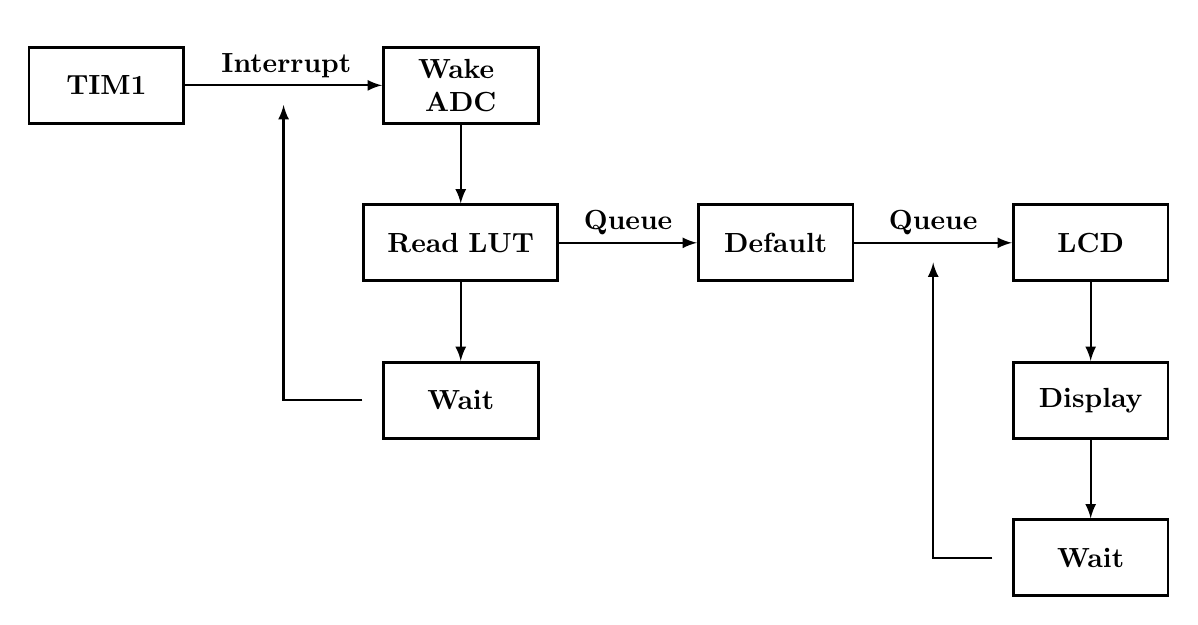
\begin{tikzpicture}[transform shape]
	\node[shape=rectangle, draw, line width=1pt, minimum width=1.965cm, minimum height=0.965cm] at (2.5, 7.5){} node[anchor=center, align=center, text width=1.577cm, inner sep=6pt] at (2.5, 7.5){$\textbf{TIM1}$};
	\node[shape=rectangle, draw, line width=1pt, minimum width=1.965cm, minimum height=0.965cm] at (7, 7.5){} node[anchor=center, align=center, text width=1.577cm, inner sep=6pt] at (7, 7.5){$\textbf{Wake }$\\$\textbf{ADC}$};
	\node[shape=rectangle, draw, line width=1pt, minimum width=2.465cm, minimum height=0.965cm] at (7, 5.5){} node[anchor=center, align=center, text width=2.077cm, inner sep=6pt] at (7, 5.5){$\textbf{Read LUT}$};
	\node[shape=rectangle, draw, line width=1pt, minimum width=1.965cm, minimum height=0.965cm] at (7, 3.5){} node[anchor=center, align=center, text width=1.577cm, inner sep=6pt] at (7, 3.5){$\textbf{Wait}$};
	\node[shape=rectangle, draw, line width=1pt, minimum width=1.965cm, minimum height=0.965cm] at (11, 5.5){} node[anchor=center, align=center, text width=1.577cm, inner sep=6pt] at (11, 5.5){$\textbf{Default}$};
	\draw[line width=0.8pt, -latex] (3.5, 7.5) -- (6, 7.5);
	\draw[line width=0.8pt, -latex] (8.25, 5.5) -- (10, 5.5);
	\draw[line width=0.8pt, -latex] (12, 5.5) -- (14, 5.5);
	\draw[line width=0.8pt, -latex] (7, 7) -- (7, 6);
	\draw[line width=0.8pt, -latex] (7, 5) -- (7, 4);
	\node[shape=rectangle, draw, line width=1pt, minimum width=1.965cm, minimum height=0.965cm] at (15, 5.5){} node[anchor=center, align=center, text width=1.577cm, inner sep=6pt] at (15, 5.5){$\textbf{LCD}$};
	\node[shape=rectangle, draw, line width=1pt, minimum width=1.965cm, minimum height=0.965cm] at (15, 3.5){} node[anchor=center, align=center, text width=1.577cm, inner sep=6pt] at (15, 3.5){$\textbf{Display}$};
	\node[shape=rectangle, draw, line width=1pt, minimum width=1.965cm, minimum height=0.965cm] at (15, 1.5){} node[anchor=center, align=center, text width=1.577cm, inner sep=6pt] at (15, 1.5){$\textbf{Wait}$};
	\draw[line width=0.8pt, -latex] (15, 5) -- (15, 4);
	\draw[line width=0.8pt, -latex] (15, 3) -- (15, 2);
	\node[shape=rectangle, minimum width=1.965cm, minimum height=0.965cm] at (13, 5.75){} node[anchor=center, align=center, text width=1.577cm, inner sep=6pt] at (13, 5.75){$\textbf{Queue}$};
	\node[shape=rectangle, minimum width=1.715cm, minimum height=0.965cm] at (9.125, 5.75){} node[anchor=center, align=center, text width=1.327cm, inner sep=6pt] at (9.125, 5.75){$\textbf{Queue}$};
	\node[shape=rectangle, minimum width=1.965cm, minimum height=0.965cm] at (4.75, 7.75){} node[anchor=center, align=center, text width=1.577cm, inner sep=6pt] at (4.75, 7.75){$\textbf{Interrupt}$};
	\draw[line width=0.8pt, -latex] (5.75, 3.5) -- (4.75, 3.5) -- (4.75, 7.25);
	\draw[line width=0.8pt, -latex] (13.75, 1.5) -- (13, 1.5) -- (13, 5.25);
\end{tikzpicture}
	
\end{center}	
\end{figure}


The system operates as an interrupt-driven pipeline: a periodic timer triggers the ADC, which acquires an analog signal. The raw value is converted via a LUT into meaningful data and placed in an RTOS queue. A dedicated task reads from the queue, processes the data, and notifies an LCD task, which updates the display.

\subsection{Conclusions}

The firmware correctly reads ambient temperature at 10\,Hz using an NTC thermistor. The three-task FreeRTOS architecture keeps acquisition, routing, and display concerns fully separated. The event-flag mechanism makes sure the acquisition task is woken exclusively by the TIM1 interrupt and waits for both ADC conversions to complete before computing the result, avoiding  busy-waiting. Temperature is encoded as \texttt{uint16\_t} $= 10\times T_K$, allowing one decimal digit to be stored in an integer type and displayed on the four-digit LCD.


\end{document}





